%!TEX program = xelatex
\documentclass[a4paper, UTF8]{ctexrep}
\usepackage{ctex}
\usepackage{amsmath}
\usepackage{multirow}
\usepackage{amssymb}
\usepackage{graphicx}
\usepackage{geometry}
\usepackage{bm}
\usepackage{subfigure}
\usepackage{float}
\usepackage{algorithm}
\usepackage{algorithmic}

\renewcommand\thesection{\arabic{section}}

\begin{document}
	\begin{titlepage}
		\centering
		\vspace{6cm}
		\LARGE{图像处理中的数学方法第三次作业报告}\\
		\vspace{3cm}
		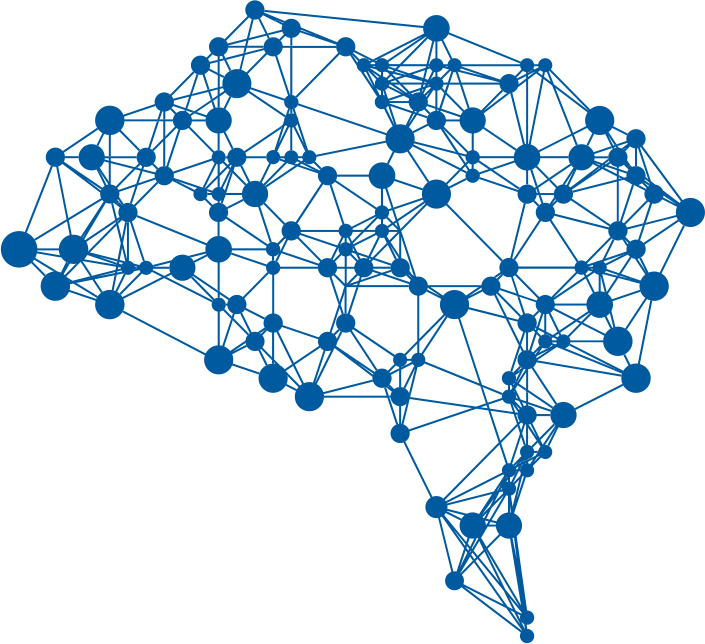
\includegraphics[width=0.8\textwidth]{deepLearning.png}\\
		\vspace{4cm}
		\normalsize{安捷 1601210097}\\
		\normalsize{\today}
	\end{titlepage}
	\section{算法描述}
		在这一次作业中,我实现了使用level set公式的Geodesic active contour模型,并利用我实现的代码,研究了不同测试图像下算法的结果、算法对参数的敏感性、算法受到图像噪声/模糊的影响、算法reinitialaton设置等问题,并且在本文中我讲叙述我在实现模型并进行数值实验中的一些感受与疑问。
		\subsubsection{算法流程} % (fold)
		\label{ssub:算法流程}
			\begin{algorithm}
				\caption{Geodesic Active Contour with Level Set}
				\begin{algorithmic}
					\item[1] 导入图像,并对图像做进行double化,归一化,对于多通道图像进行rgb2gray,权衡计算速度调整图像大小;
					\item[2] 对图像进行灰度值scale,使得图像灰度为分布于$\left(0, 255\right)$之间的double数;(增强图像对比度,加强梯度信息的强度,为level set做预处理)	
					\item[3] 对图像添加模糊或噪声;(用于观察图像噪声或模糊对结果的影响,不对此进行数值实验时可以忽略)
					\item[4] 算法初始化,计算单步迭代步长,设置迭代次数上限及各种参数;
					\item[5] 按照公式$\frac{\partial v}{\partial t} = g\left(|\nabla I|\right)|\nabla v|\mathrm{div} \left(\frac{\nabla v}{|\nabla v|}\right) + \alpha g \left( |\nabla I| \right) |\nabla v| + \nabla g \cdot \nabla v$开始迭代;
					\item[6] 每次更新$v$之后执行10步reinitialization;
					\item[7] 迭代结束,显示图像,保存结果;
				\end{algorithmic}
			\end{algorithm}
		
		\subsubsection{算法实现的准备} % (fold)
			在实现算法之前,我自行构造了一张测试图像用于验证算法的正确性,测试图像如下:\clearpage
			\begin{figure}[htbp!]
				\centering
				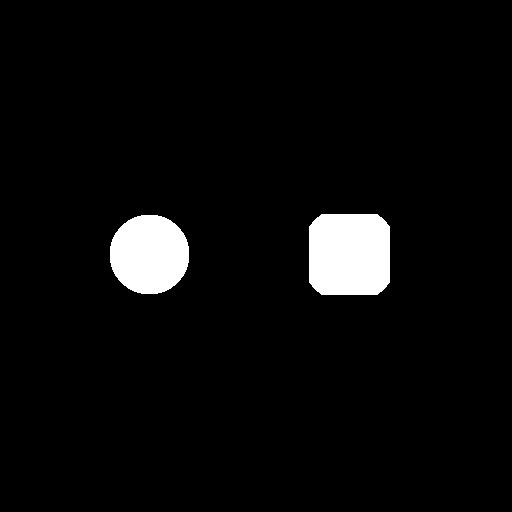
\includegraphics[width=0.8\textwidth]{hw3_fig1.jpg}
				\caption{人工构造的测试图像}
				\label{fig:figure1}
			\end{figure}
		
		% subsubsection  (end)
		\subsubsection{MATLAB子函数功能说明} % (fold)
		\label{ssub:matlab子函数功能说明}
			\begin{table}[htbp!]
				\centering
				\begin{tabular}{ll}
					\hline
					函数名称 & 函数功能 \\
					\hline
					geodesic\_active\_contour\_with\_level\_set.m & 算法实现主脚本 \\
					create\_naive\_test\_image.m & 人工测试图像生成函数 \\
					initialization\_level\_set.m & 水平集函数初始化函数 \\
					g.m & 算法迭代公式中的g函数 \\
					Reinitial2D.m & reinitialization函数 \\
					\hline
				\end{tabular}
			\end{table}
		
		% subsubsection matlab子函数功能说明 (end)
		\subsubsection{参数名称及功能} % (fold)
		\label{ssub:参数名称及功能}
			\begin{table}[htbp!]
				\centering
				\begin{tabular}{lll}
					\hline
					参数名称 & 参数功能 & 参数推荐值 \\
					\hline
					IMG\_PATH & 图像路径 &   \\
					SIGMA & 图像高斯模糊参数 & 4 \\
					NOISE\_SCALE & 图像高斯噪声参数 & 50 \\
					MAX\_ITERATION & 最大迭代次数 & 1000 \\
					STEP\_SIZE & 单步迭代步长 & 0.5/(max(row,col)-1) \\
					ALPHA & 迭代公式第二项权重 & 800 \\
					BETA & 迭代公式第三项权重 & 200 \\
					\hline
				\end{tabular}
			\end{table}
		
		% subsubsection 参数名称及功能 (end)
	\section{数值实验结果及讨论} % (fold)
	\label{sec:数值实验结果及讨论}
		\subsubsection{针对不同测试图像的数值实验结果及对应参数} % (fold)
		\label{ssub:针对不同测试图像的数值实验结果及对应参数}
			\begin{figure}[htbp!]
				\centering
				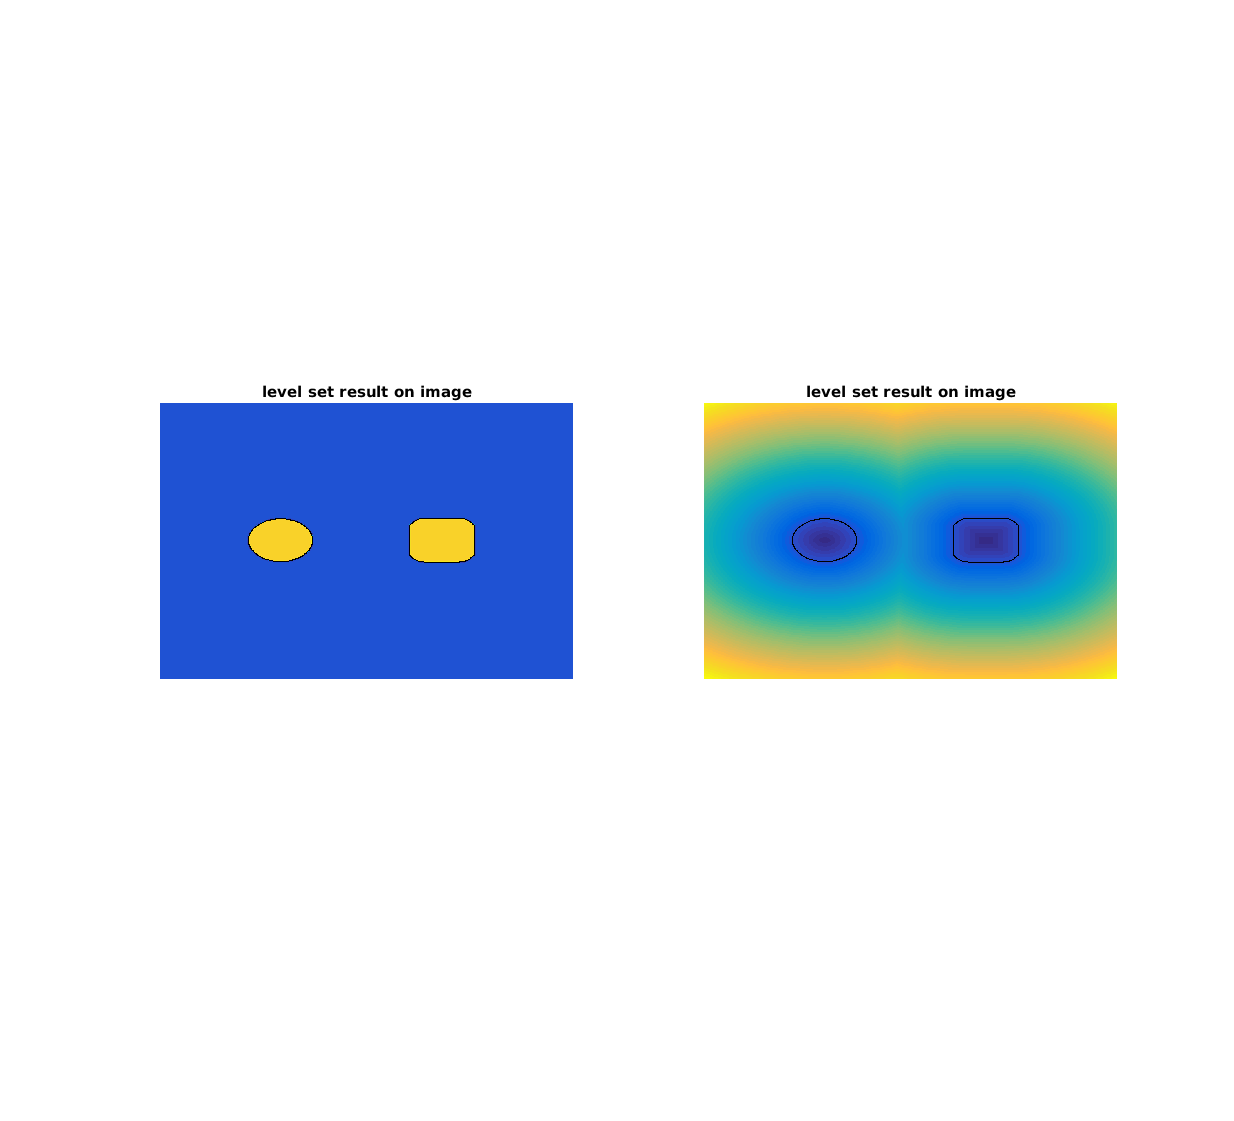
\includegraphics[width=\textwidth]{hw3_fig2.png}
				\caption{ALPHA=800,BETA=200,ITETARION=1000}
				\label{fig:figure1}
			\end{figure}
			\begin{figure}[htbp!]
				\centering
				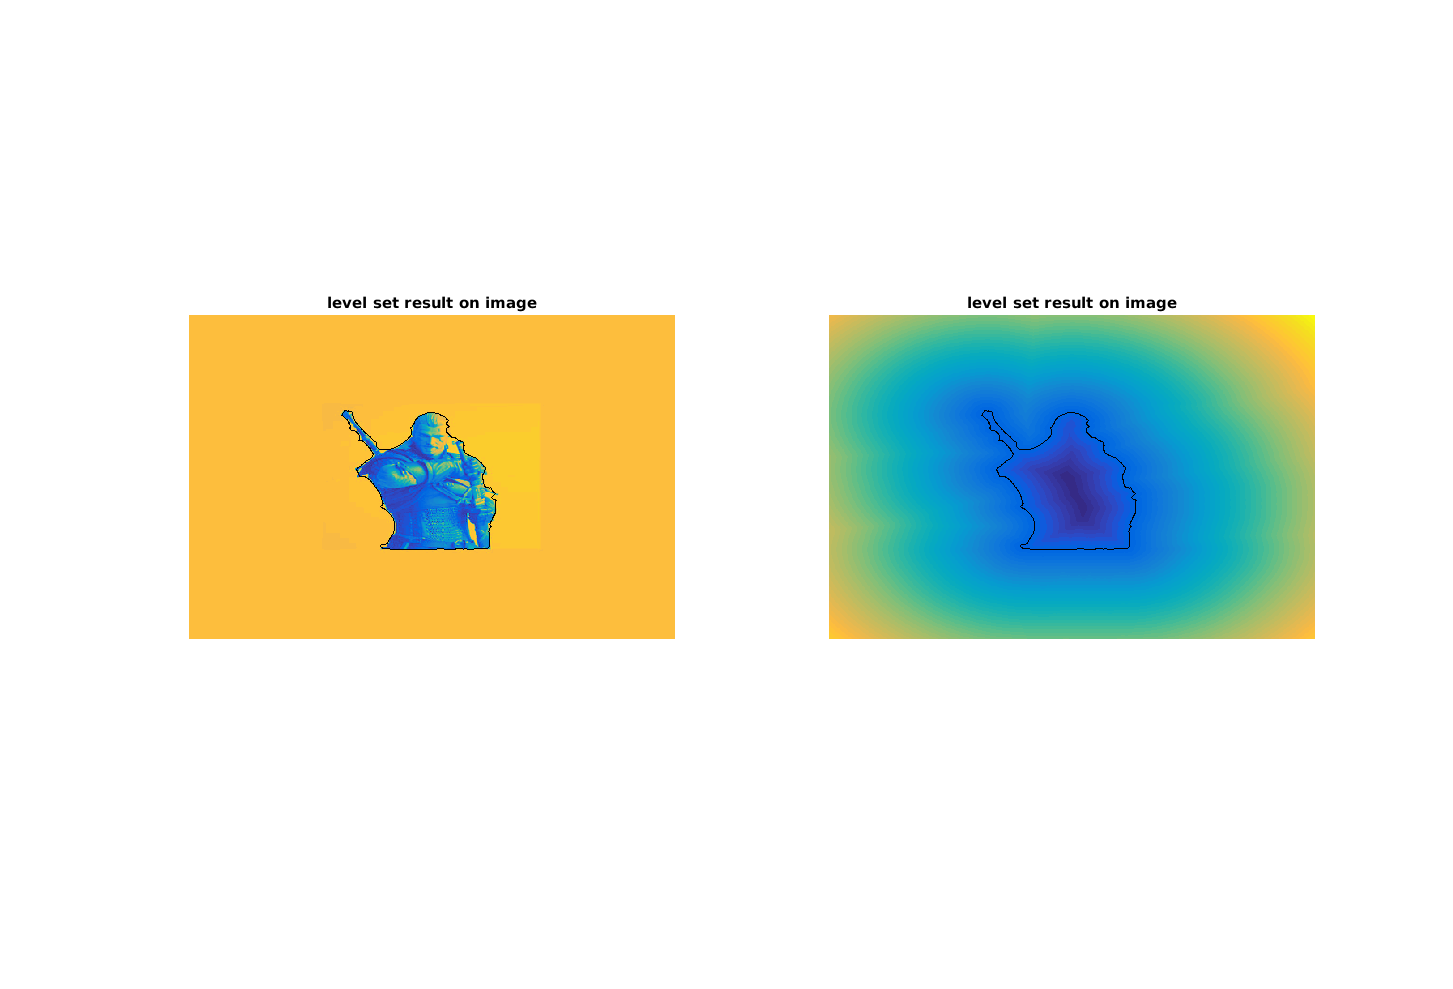
\includegraphics[width=\textwidth]{hw3_fig3.png}
				\caption{ALPHA=800,BETA=200,ITETARION=1000}
				\label{fig:figure1}
			\end{figure}
			\begin{figure}[htbp!]
				\centering
				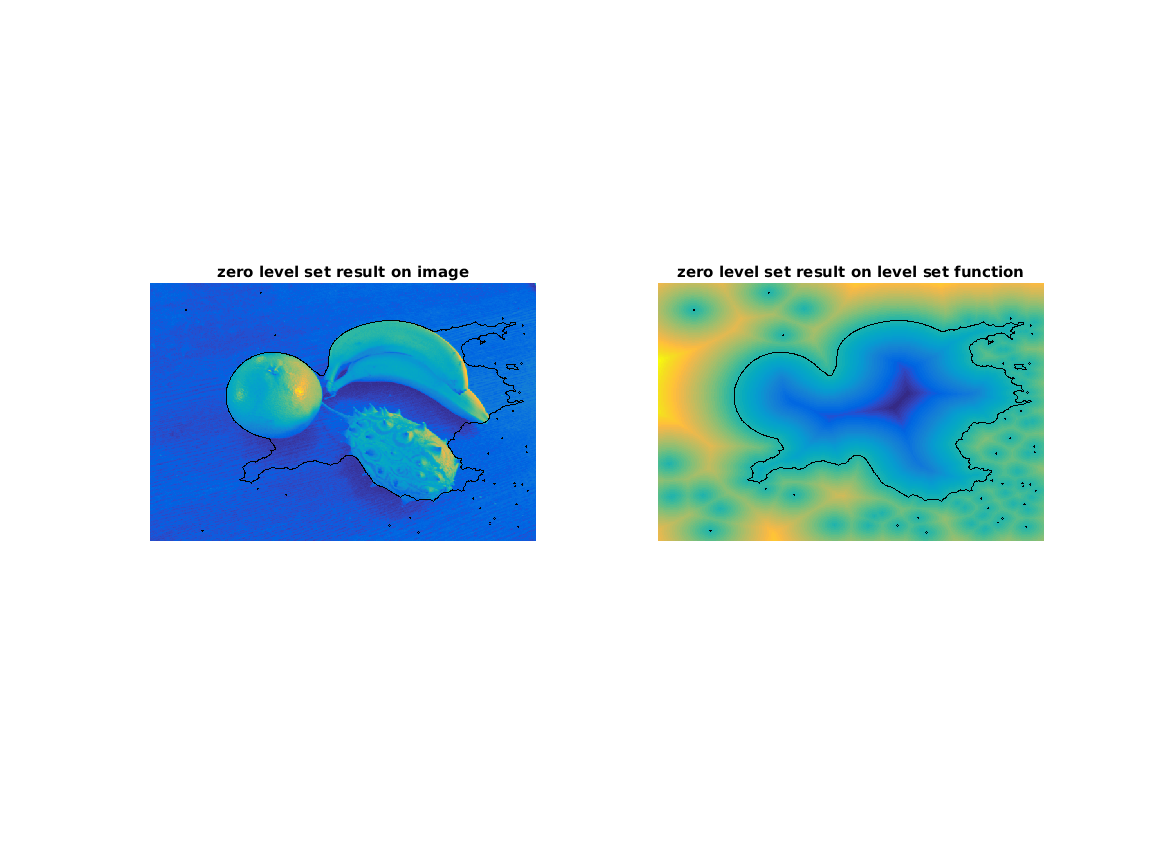
\includegraphics[width=\textwidth]{hw3_fig4.png}
				\caption{ALPHA=800,BETA=200,ITETARION=800}
				\label{fig:figure1}
			\end{figure}
			\begin{figure}[htbp!]
				\centering
				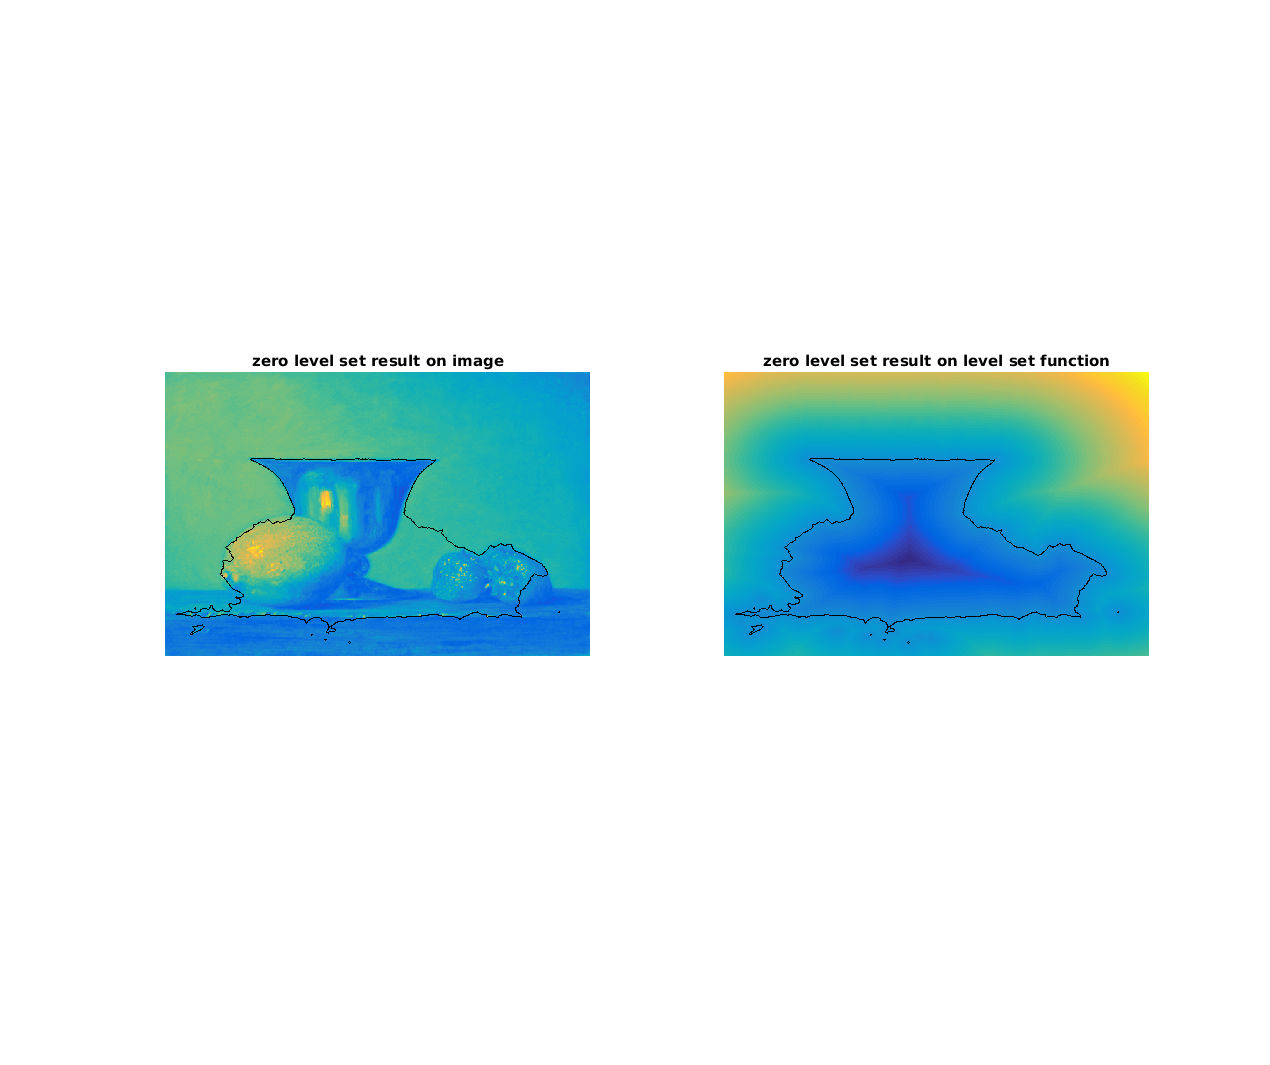
\includegraphics[width=\textwidth]{hw3_fig5.png}
				\caption{ALPHA=800,BETA=200,ITETARION=800}
				\label{fig:figure1}
			\end{figure}
			\begin{figure}[htbp!]
				\centering
				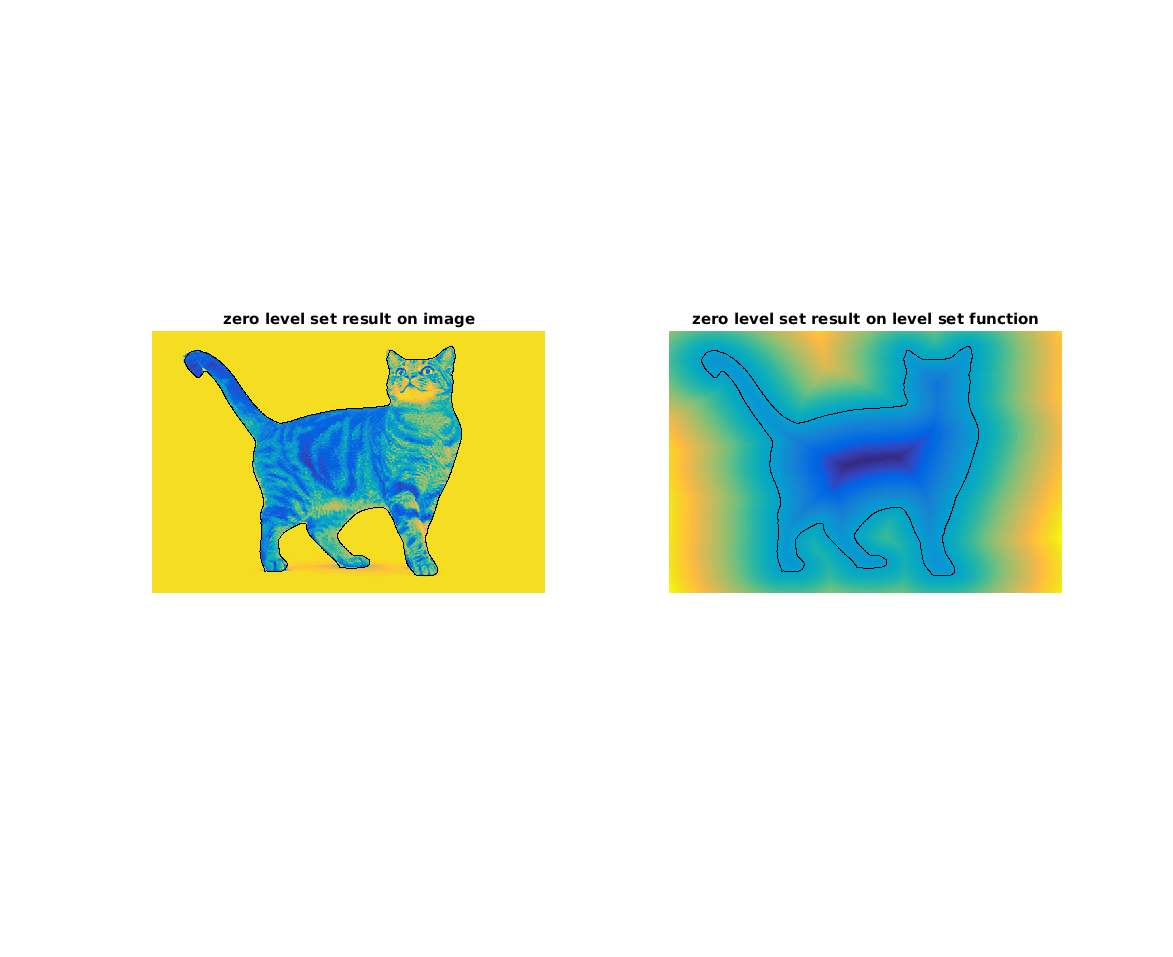
\includegraphics[width=\textwidth]{hw3_fig6.png}
				\caption{ALPHA=800,BETA=200,ITETARION=500}
				\label{fig:figure1}
			\end{figure}
			\begin{figure}[htbp!]
				\centering
				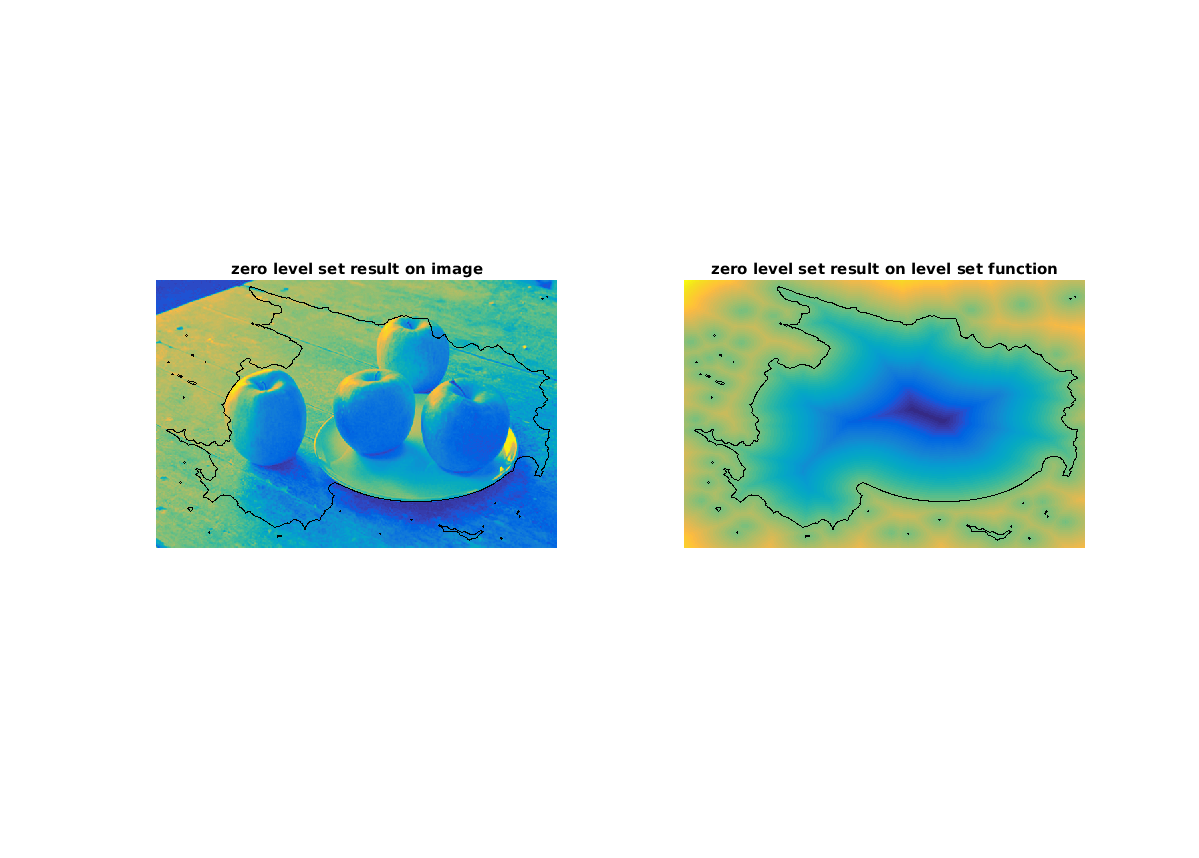
\includegraphics[width=\textwidth]{hw3_fig7.png}
				\caption{ALPHA=800,BETA=100,ITETARION=1500}
				\label{fig:figure1}
			\end{figure}
			\begin{figure}[htbp!]
				\centering
				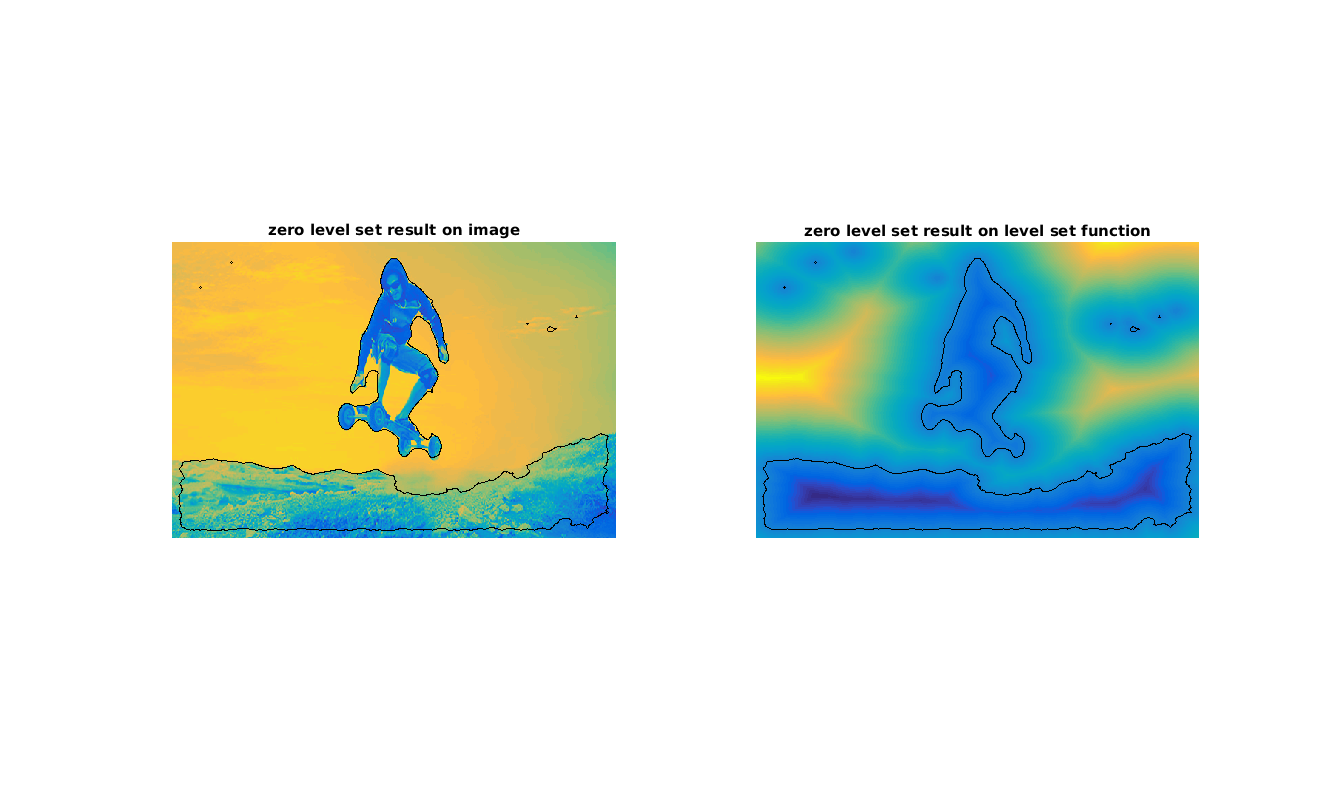
\includegraphics[width=\textwidth]{hw3_fig8.png}
				\caption{ALPHA=800,BETA=200,ITETARION=800}
				\label{fig:figure1}
			\end{figure}
			\clearpage
		% subsubsection 针对不同测试图像的数值实验结果及对应参数 (end)
	% section 数值实验结果及讨论 (end)

		% subsubsection 算法流程 (end)
		\subsubsection{图像灰度值scale作用} % (fold)
		\label{ssub:图像灰度值scale说明}
			经过了若干次数值实验,我观察到,当图像归一化为$\left( 0,1 \right)$之间的double数时,由于梯度的值过小,图像信息对于水平集函数的演化贡献太小,导致水平集函数完全忽略了图像的边界,直接不断升高直至零水平集消失,结果如下图所示
			\begin{figure}[htbp!]
				\centering
				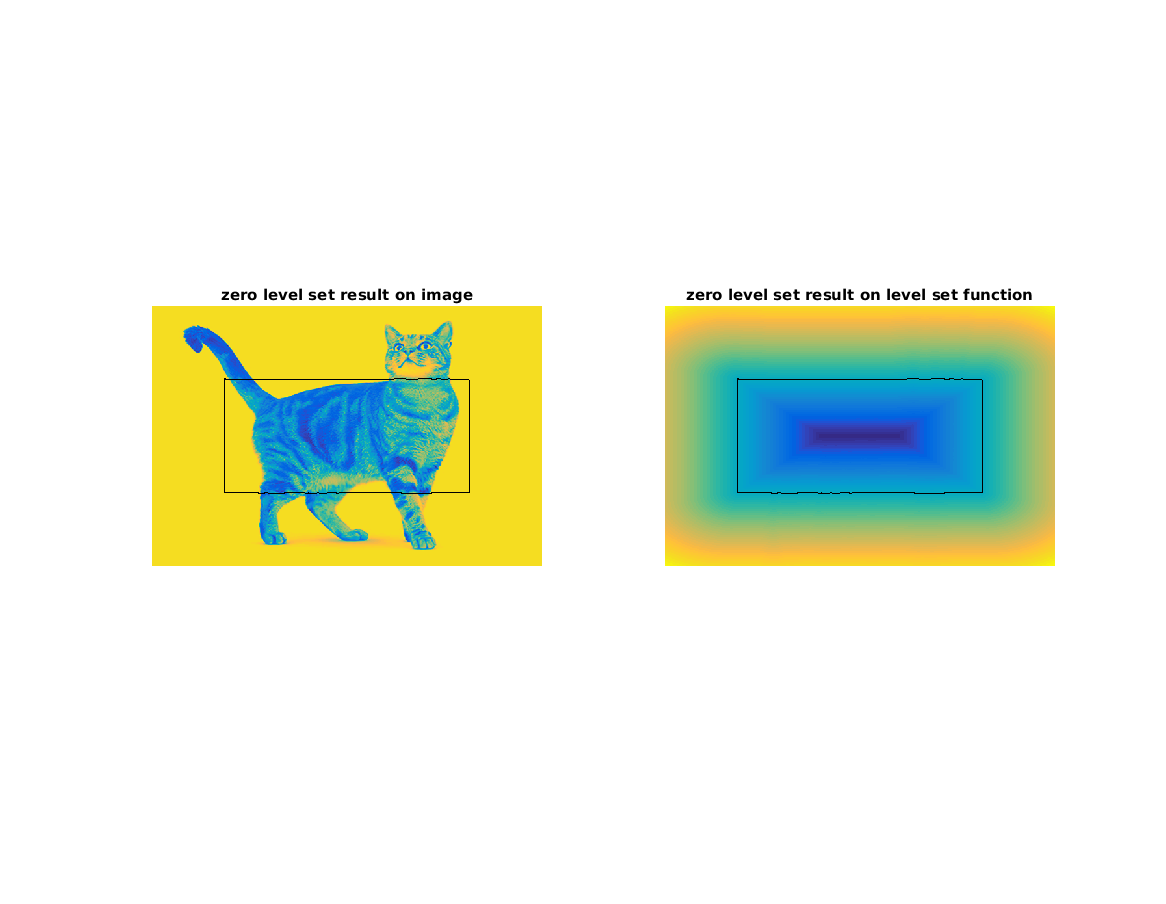
\includegraphics[width=\textwidth]{hw3_fig9.png}
				\caption{ALPHA=800,BETA=200,ITETARION=150,without itensity scale}
				\label{fig:figure1}
			\end{figure}
			\clearpage
		% subsubsection 图像灰度值scale说明 (end)
		\subsubsection{初始水平集函数形状对结果的影响} % (fold)
		\label{ssub:初始水平集函数形状对结果的影响}
			经过数值实验,我发现,对于圆形与方形的初始水平集函数,算法都能正常运行并且得到可靠的结果,在initialization\_level\_set.m中我分别写了圆形与方形的初始化代码,最终使用方形的原因是方形可以更好的保证待分割主体能够位于零水平集内部,圆形初始化的中间过程如下图:
			\begin{figure}[htbp!]
				\centering
				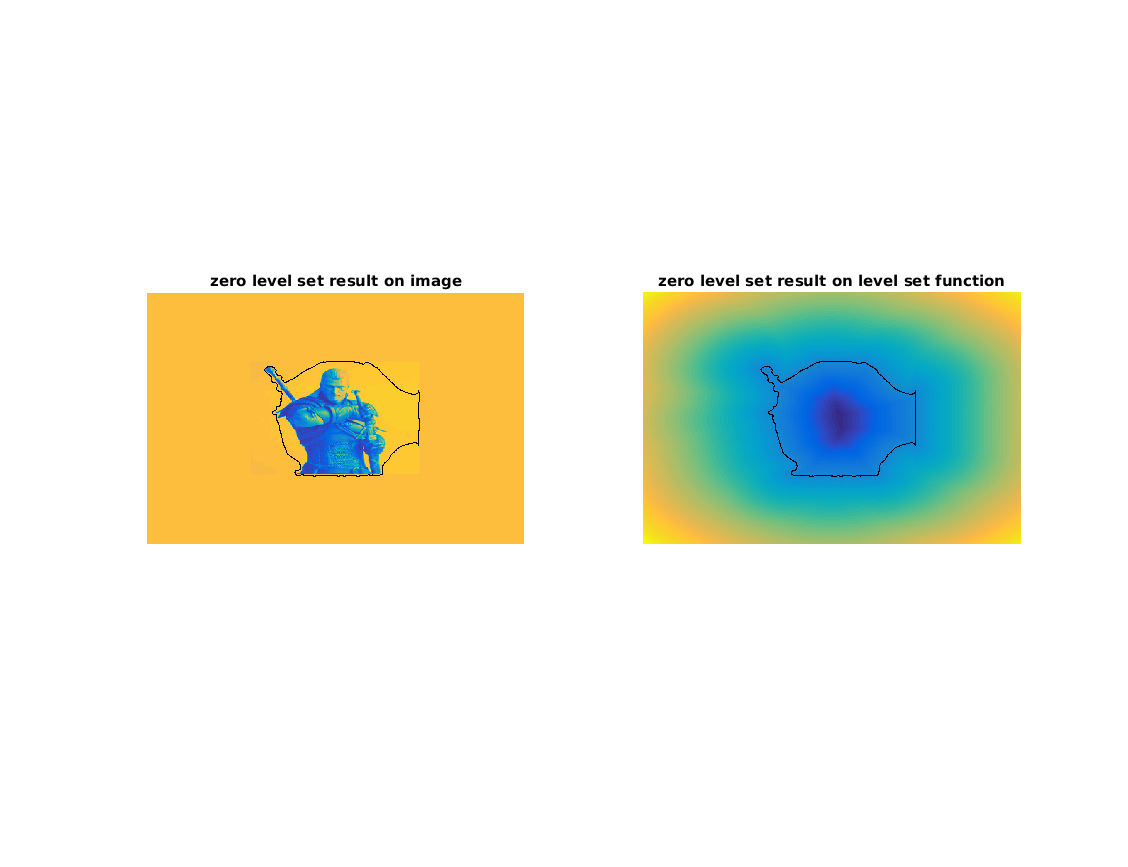
\includegraphics[width=\textwidth]{hw3_fig10.png}
				\caption{ALPHA=800,BETA=200,ITETARION=200}
				\label{fig:figure1}
			\end{figure}
			\clearpage
		% subsubsection 初始水平集函数形状对结果的影响 (end)
		\subsubsection{关于ALPHA,BETA作用的探讨} % (fold)
		\label{ssub:关于_}
			经过若干次数值实验,我感觉到,ALPHA主要会影响算法的收敛速度,即水平集函数收缩的快慢,越大的ALPHA可以使得函数尽早收敛,BETA起到的作用是加强边缘信息对水平集函数收敛过程的影响,形象的说,BETA越大,边缘对水平集函数的拉力就越大,但是BETA的增大也会造成负面作用,即图像背景的噪声或一些无关紧要的细节被分割出来,与此同时,BETA的增大还会略微降低水平集函数的收敛速度。
		% subsubsection 关于_ (end)

		\subsubsection{图像模糊和噪声对结果的影响} % (fold)
		\label{ssub:图像模糊对结果的影响}
			图像模糊对于本来就有均匀背景,容易分割的图像会使得图像分割结果产生边角上细节的丢失,如下图:
			\begin{figure}[htbp!]
				\centering
				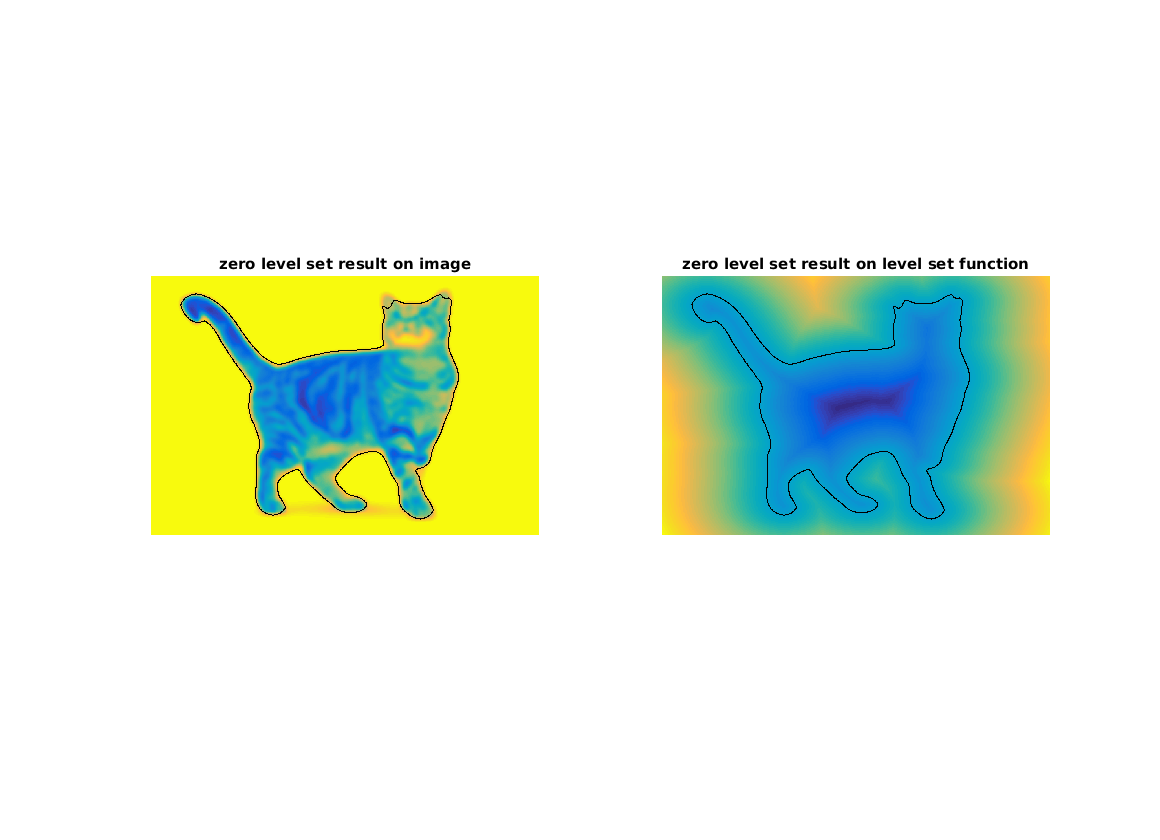
\includegraphics[width=\textwidth]{hw3_fig11.png}
				\caption{ALPHA=800,BETA=200,ITETARION=500}
				\label{fig:figure1}
			\end{figure}
			\clearpage
			但是,对于背景噪声很强的图像,平滑能够起到一定去噪但是保留主体的作用,增强分割的结果,并且能够加快这种情况下的收敛速度,如下图:
			\begin{figure}[htbp!]
				\centering
				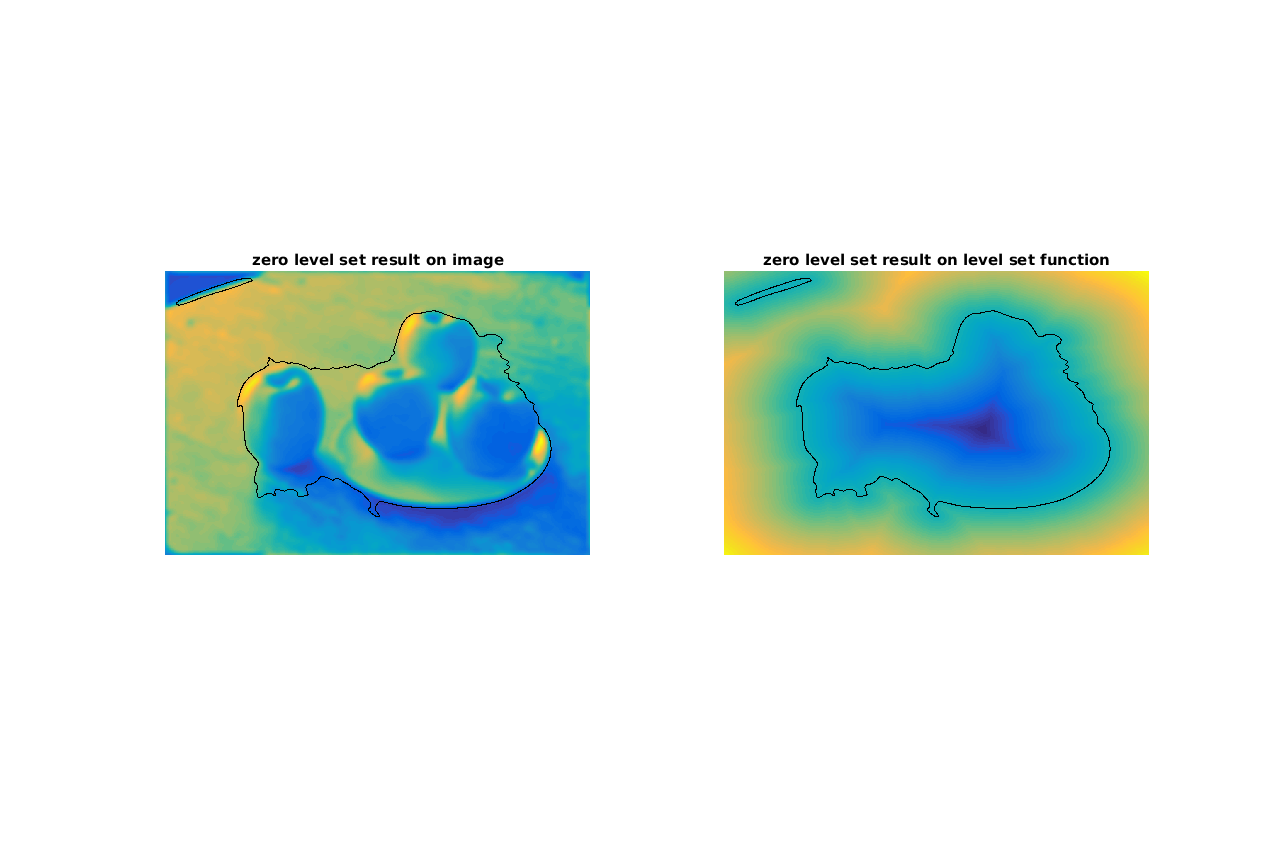
\includegraphics[width=\textwidth]{hw3_fig12.png}
				\caption{ALPHA=800,BETA=200,ITETARION=300}
				\label{fig:figure1}
			\end{figure}
			\clearpage
			噪声与之相比,会起到相反的作用,即使得图像分割的结果变差,并且会大幅拖慢收敛速度,如下图:
			\begin{figure}[htbp!]
				\centering
				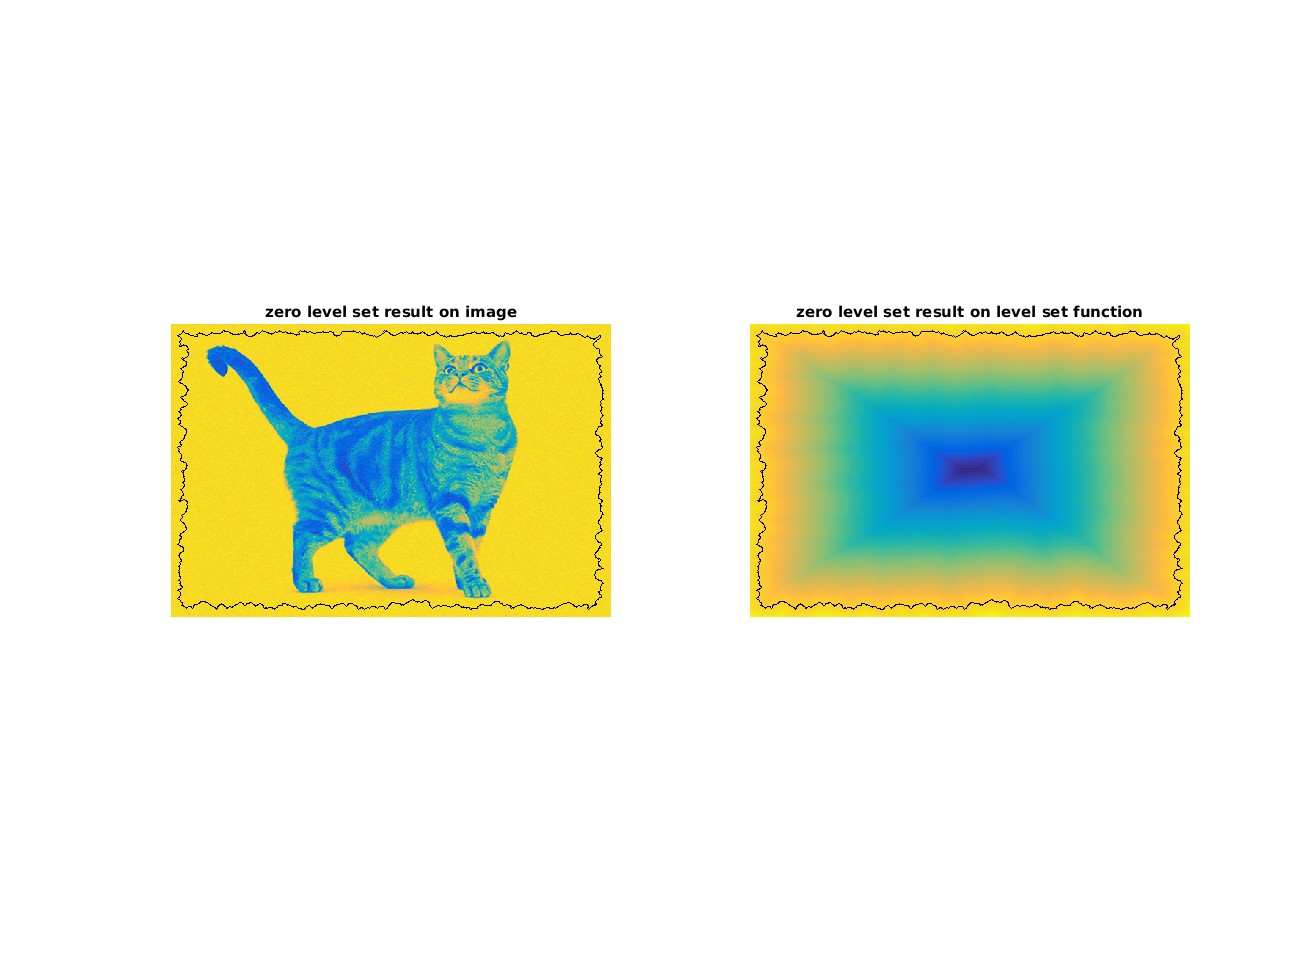
\includegraphics[width=\textwidth]{hw3_fig13.png}
				\caption{ALPHA=800,BETA=200,ITETARION=500}
				\label{fig:figure1}
			\end{figure}

		% subsubsection 图像模糊对结果的影响 (end)
		\subsubsection{关于差分格式的讨论} % (fold)
		\label{ssub:关于差分格式的讨论}
			在这一次作业中,ppt中要求使用迎风格式进行差分运算,我在实现的过程中分别尝试使用了迎风格式与一般差分格式,二者的结果没有明显可见的显著差别,考虑到计算的速度我注释掉了迎风格式的代码使用了速度更快的一般差分格式,因此我有疑惑:
			\begin{enumerate}
				\item 迎风格式的作用是什么?
				\item 什么时候必须使用迎风格式?即不使用则不能得到正确的结果,什么情况下一般差分与迎风格式没有显著差别?
			\end{enumerate}
		% subsubsection 关于差分格式的讨论 (end)
		\subsubsection{关于reinitialization的讨论} % (fold)
		\label{ssub:关于reinitialization的讨论}
			这一次作业中最令我感到意外的是,算法的结果非常依赖于reinitialization的介入,具体表现为:
			\begin{enumerate}
				\item 每迭代10步使用一次reinitialization并进行10次reinit迭代,则算法不收敛,不能得到有意义的结果;
				\item 每次迭代都进行10步reinit操作即可得到非常正常且有效的结果;
			\end{enumerate}
			因此通过数值实验我认识到了算法对于reinitialization的巨大依赖且非常敏感。
		% subsubsection 关于reinitialization的讨论 (end)
		\subsubsection{关于实现方法的讨论} % (fold)
		\label{ssub:关于实现方法的讨论}
			在之前学习工科版的图像处理的过程中我也接触过level set算法,在工科版的教材中,level set算法一般有两项,第一项为梯度项,主要作用为促进水平集函数收缩,并且,\textbf{这一项只与水平集函数相关而与直接的图像信息无关},第二项为内外能量项,通过边缘信息约束水平集函数的收缩,这一种实现方法也可以实现水平集算法,因此我猜测算法对于g的选取及前两项(即工科中的梯度项)中图像信息直接参与不敏感。
		% subsubsection 关于实现方法的讨论 (end)
	\section{总结} % (fold)
	\label{sec:总结}
		这一次作业中,我实现了Geodesic active contour with level set formula算法,并进行了若干数值实验,总的来说,收获很多,不过也有很多疑问,尤其是关于迎风格式的疑问,可以说这一疑问在之前几次作业的实现中也有,这一次最为强烈,因此不知能否麻烦助教稍微给我解释一下相关的内容?谢谢助教老师~ 
	% section 总结 (end)

	    

\end{document}